% !TeX spellcheck = en_US
% !TeX encoding = UTF-8
\section{Enveloping Distribution Sampling\label{Sec:ES:EDS}}
Enveloping distribution sampling method was first proposed by Christ and van Gunsteren in 2007.\cite{ChristJCP2007}
When calculating the free energy difference between states $A$ and $B$,
\begin{equation}
	\Delta G_{BA}=G_B-G_A=-\beta^{-1}\ln{\frac{Q_B}{Q_A}},
\end{equation}
we may encounter convergence difficulty if the important spaces of these two states are well separated, shown as black lines in Fig.~\ref{Fig:ES:triple_gaussian}.
Simulation under the Hamiltonian of state $A$ can hardly cover the important region of Hamiltonian $B$, and then the free energy of state $B$ will be significantly overestimated.
\begin{figure}[htbp]
	\centering
	%	\resizebox{2cm}{!}{
	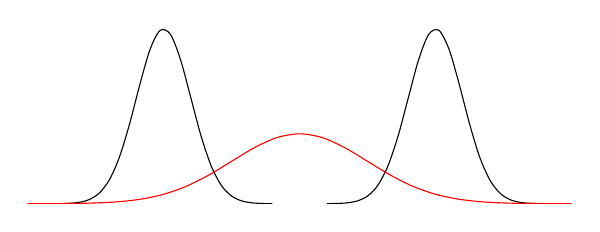
\begin{tikzpicture}
	\def\lims{xmin=-10,xmax=10,ymin=0.0001,ymax=0.6}
	\begin{axis}[\lims,hide x axis, hide y axis,width=0.7\textwidth,height=0.35\textwidth]
	    \addplot[mark=none,smooth,domain=-10:-1,y domain=0.0001:1] {0.5*exp(-(x+5)*(x+5)/2)};
		\addplot[mark=none,smooth,domain=1:10,y domain=0.0001:1] {0.5*exp(-(x-5)*(x-5)/2)};
		\addplot[color=red,mark=none,smooth,domain=-10:10,y domain=0.0001:1] {0.2*exp(-x*x/12.5)};
	\end{axis}
	\end{tikzpicture}
	%	}
	\caption{The configuration distributions under two Hamiltonians have no visible overlap as shown by solid black curves. A reference state (shown as the red curve) that has remarkable overlap with both states can be introduced to accelerate the convergence of the free energy calculations using, for instance, TP.}\label{Fig:ES:triple_gaussian}
\end{figure}

%\begin{figure}[htbp]
%	\centering
%	\includegraphics[width=0.6\textwidth]{figures/triple_gaussian.pdf}\\
%	\caption{The configuration distributions under two Hamiltonians have no visible overlap as shown by solid black curves. A reference state (shown as the red curve) that has remarkable overlap with both states can be introduced to accelerate the convergence of the free energy calculations using, for instance, TP.}\label{Fig:ES:triple_gaussian}
%\end{figure}
A simple solution to this difficulty is ``overlap sampling'', in which a reference state that can cover the important regions of both Hamiltonians $A$ and $B$ is introduced.
We then carry out a simulation for the reference state and the free energy difference between state $A$ and $B$ can be calculated as
\begin{equation}
	\Delta G_{BA}=\Delta G_{BR}-\Delta G_{AR}=-\beta^{-1}\ln{\dfrac{\langle e^{-\beta\left(H_B-H_R\right)}\rangle_R}{\langle e^{-\beta\left(H_A-H_R\right)}\rangle_R}},
\end{equation} 
which is a combination of two thermodynamic perturbation calculations from the reference state to the target states.

However, building the Hamiltonian of the reference state is not trivial. Without knowledge of the Hamiltonians for state $A$ and state $B$, we cannot generate an effective Hamiltonian,
especially in a high dimensional space. Enveloping distribution sampling method provides a natural way to generate the Hamiltonian for the reference state with simply mixing the Hamiltonians of state $A$ and state $B$ in the following way
\begin{equation}
	H_R(\mathbf{r})=-\left(s\beta\right)^{-1}\ln{\left(e^{-s\beta H_A(\mathbf{r})}+e^{-s\beta H_B(\mathbf{r})}\right)},
	\label{Eq:ES:EDS:H_R}
\end{equation}
where $s$ is a scale factor that modulates the mixing\cite{ChristJCTC2009} as shown in Fig.~\ref{Fig:ES:EDS}. Increasing $s$ lowers the barrier height separating the two minima in the mixed potential, thereby enhances the transition. Straightforwardly, you may come to the idea that running Hamiltonian-REMD with different $s$ can remarkably increase the efficiency.
If you take a close look at Eq.~\ref{Eq:ES:EDS:H_R}, you will find that $s$ appears always with $\beta$. In other words, changing $s$ is equivalent to changing the temperature for the simulation. This is one interesting case where H-REMD and T-REMD are coincident with each other. 
\begin{figure}[htbp]
	\centering
	%	\resizebox{2cm}{!}{
	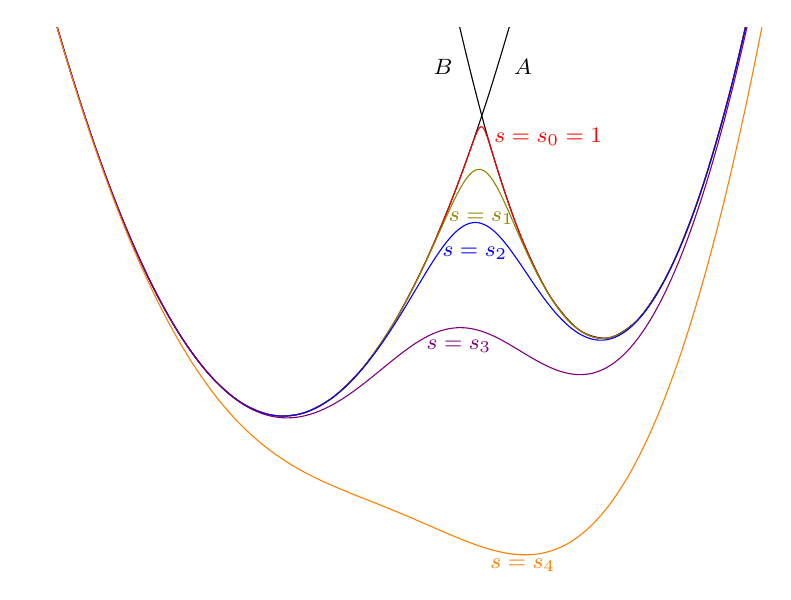
\begin{tikzpicture}
	\def\lims{xmin=-13,xmax=10,ymin=-20,ymax=50}
	\begin{axis}[\lims,hide x axis, hide y axis,width=0.9\textwidth,height=0.7\textwidth]
	\addplot[mark=none,smooth,domain=-13:10] {(x+5)*(x+5)};
	\addplot[mark=none,smooth,domain=-13:10] {10+2*(x-5)*(x-5)};
	\addplot[color=red,mark=none,samples=500,domain=-13:10] { -2*ln(exp(-0.5*(x+5)*(x+5))+exp(-0.5*(10+2*(x-5)*(x-5))))};
	\addplot[color=olive,mark=none,samples=500,domain=-13:10] {-10*ln(exp(-0.1*(x+5)*(x+5))+exp(-0.1*(10+2*(x-5)*(x-5))))};
	\addplot[color=blue,mark=none,samples=500,domain=-13:10] {-20*ln(exp(-0.05*(x+5)*(x+5))+exp(-0.05*(10+2*(x-5)*(x-5))))};
	\addplot[color=violet,mark=none,samples=500,domain=-13:10] {-40*ln(exp(-0.025*(x+5)*(x+5))+exp(-0.025*(10+2*(x-5)*(x-5))))};
	\addplot[color=orange,mark=none,samples=500,domain=-13:10] {-80*ln(exp(-0.0125*(x+5)*(x+5))+exp(-0.0125*(10+2*(x-5)*(x-5))))};
    \node[] at (axis cs: 2.5,45) {\footnotesize$A$};
    \node[] at (axis cs: 0.0,45) {\footnotesize$B$};
    \node[color=red] at (axis cs: 3.3,36) {\footnotesize$s=s_0=1$};
    \node[color=olive] at (axis cs: 1.2,25.5) {\footnotesize$s=s_1$};
    \node[color=blue] at (axis cs: 1.0,21) {\footnotesize$s=s_2$};
    \node[color=violet] at (axis cs: 0.5,9) {\footnotesize$s=s_3$};
    \node[color=orange] at (axis cs: 2.5,-19.2) {\footnotesize$s=s_4$};
	\end{axis}
	\end{tikzpicture}
	%	}
	\caption{State A and state B have only negligible overlap at high energy regions. The reference state generated by the mixing of state A and state B is characterized by $s$. Increasing $s$ may lower the barrier between the dominant wells.}\label{Fig:ES:EDS}
\end{figure}

%\begin{figure}[htbp]
%	\centering
%	\includegraphics[width=0.8\textwidth]{figures/EDS.pdf}\\
%	\caption{State A and state B have only negligible overlap at high energy regions. The reference state generated by the mixing of state A and state B is characterized by $s$. Increasing $s$ may lower the barrier between the dominant wells.}\label{Fig:ES:EDS}
%\end{figure}

The force is also a mixing quantity from two Hamiltonians as
\begin{align}
	\mathbf{F}_R^i=-\frac{\partial H_R}{\partial \mathbf{r}^i}=&\frac{e^{-s\beta H_A(\mathbf{r})}}{e^{-s\beta H_A(\mathbf{r})}+e^{-s\beta H_B(\mathbf{r})}}\left(-\frac{\partial H_A(\mathbf{r})}{\partial \mathbf{r}^i}\right)\notag\\
	&+\frac{e^{-s\beta H_B(\mathbf{r})}}{e^{-s\beta H_A(\mathbf{r})}+e^{-s\beta H_B(\mathbf{r})}}\left(-\frac{\partial H_B(\mathbf{r})}{\partial \mathbf{r}^i}\right).
\end{align}
